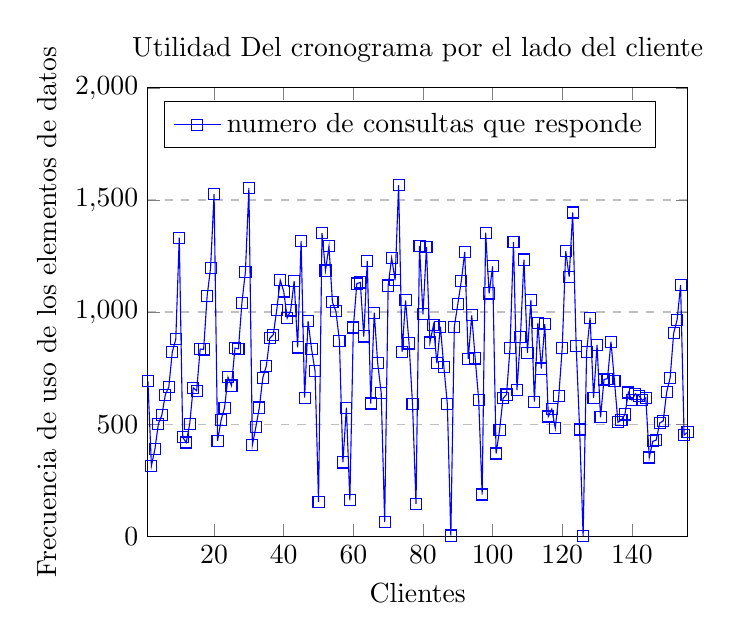
\begin{tikzpicture}
\begin{axis}[
    title={Utilidad Del cronograma por el lado del cliente},
    xlabel={Clientes},
    ylabel={Frecuencia de uso de los elementos de datos},
    xmin=1, xmax=156,
    ymin=0, ymax=2000,
    xtick={},
    ytick={},
    legend pos=north west,
    ymajorgrids=true,
    grid style=dashed,
]

\addplot[
    color=blue,
    mark=square,
    ]
    coordinates {
        %UTILIDAD DE ELEMENTOS EXATCTOS
%(cronograma, numero consultas exactas que usan al cronograma)
(1,691)
(2,314)
(3,388)
(4,501)
(5,540)
(6,631)
(7,666)
(8,822)
(9,879)
(10,1332)
(11,441)
(12,418)
(13,501)
(14,662)
(15,649)
(16,835)
(17,833)
(18,1071)
(19,1198)
(20,1526)
(21,425)
(22,517)
(23,573)
(24,709)
(25,672)
(26,839)
(27,836)
(28,1042)
(29,1180)
(30,1554)
(31,407)
(32,487)
(33,574)
(34,707)
(35,759)
(36,883)
(37,899)
(38,1009)
(39,1142)
(40,1092)
(41,973)
(42,1007)
(43,1138)
(44,842)
(45,1317)
(46,618)
(47,959)
(48,835)
(49,737)
(50,153)
(51,1352)
(52,1185)
(53,1293)
(54,1043)
(55,1003)
(56,872)
(57,329)
(58,573)
(59,160)
(60,931)
(61,1127)
(62,1132)
(63,891)
(64,1228)
(65,592)
(66,997)
(67,771)
(68,640)
(69,63)
(70,1118)
(71,1241)
(72,1142)
(73,1566)
(74,822)
(75,1052)
(76,860)
(77,589)
(78,144)
(79,1295)
(80,990)
(81,1289)
(82,864)
(83,941)
(84,771)
(85,935)
(86,756)
(87,589)
(88,3)
(89,934)
(90,1035)
(91,1137)
(92,1268)
(93,791)
(94,985)
(95,793)
(96,609)
(97,186)
(98,1354)
(99,1083)
(100,1204)
(101,369)
(102,473)
(103,615)
(104,632)
(105,839)
(106,1312)
(107,652)
(108,890)
(109,1234)
(110,818)
(111,1054)
(112,600)
(113,952)
(114,748)
(115,946)
(116,534)
(117,567)
(118,482)
(119,624)
(120,840)
(121,1271)
(122,1158)
(123,1444)
(124,850)
(125,476)
(126,1)
(127,821)
(128,975)
(129,617)
(130,853)
(131,530)
(132,699)
(133,703)
(134,868)
(135,693)
(136,508)
(137,518)
(138,543)
(139,641)
(140,608)
(141,635)
(142,627)
(143,606)
(144,617)
(145,351)
(146,423)
(147,429)
(148,505)
(149,514)
(150,643)
(151,707)
(152,905)
(153,966)
(154,1120)
(155,451)
(156,463)

    };
    \legend{numero de consultas que responde}

\end{axis}
\end{tikzpicture}

